%%%%%%%%%%%%%%%%%%%%%%%%%%%%%%%%%%%%%%%%%%%%%%%%%%%%%%%%%%%%%%%
%%%  notes
%%%%%%%%%%%%%%%%%%%%%%%%%%%%%%%%%%%%%%%%%%%%%%%%%%%%%%%%%%%%%%%

\documentclass[onecolumn,fleqn,notitlepage,secnumarabic]{revtex4}

% Text arrangement

\newcommand{\rmrk}[1]{\textcolor{red}{#1}}
\newcommand{\Eq}[1]{\textcolor{blue}{Eq.\!\!~(\ref{#1})}} 
\newcommand{\Fig}[1]{\textcolor{blue}{Fig.}\!\!~\ref{#1}}
\newcommand{\drawline}{\begin{picture}(500,1)\line(1,0){500}\end{picture}}
\newcommand{\bitem}{$\bullet$ \ \ \ }
\newcommand{\Cn}[1]{\begin{center} #1 \end{center}}
\newcommand{\mpg}[2][1.0\hsize]{\begin{'}[b]{#1}{#2}\end{'}}
\newcommand{\mpgt}[2][1.0\hsize]{\begin{'}[t]{#1}{#2}\end{'}}


% special 
\usepackage{ifthen}
\usepackage{ifpdf}
\usepackage{float}
\usepackage{color}

% fonts
\usepackage{latexsym}
\usepackage{amsmath} 
\usepackage{amssymb} 
\usepackage{bm}
\usepackage{wasysym}


\ifpdf
\usepackage{graphicx}
\usepackage{epstopdf}
\else
\usepackage{graphicx}
\usepackage{epsfig}
\fi

% packages added by jarondl

\usepackage{verbatim} % for multiline comments
\usepackage{natbib} % change the bibliography style 
\usepackage{fancybox} % allows putting boxes with borders
\usepackage{cmap}  % for making pdf mathmode searchable
\usepackage[pdftitle={proposal}]{hyperref}  % for hyperlinks in biblio. should be called last?

%%%%%%%%%%%%%%%%%%%%%%%%%%%%%%%%%%%%%%%%%%%%%%%%%%%%%%%%%%%%%%%%


% math symbols I
\newcommand{\sinc}{\mbox{sinc}}
\newcommand{\const}{\mbox{const}}
\newcommand{\trc}{\mbox{trace}}
\newcommand{\intt}{\int\!\!\!\!\int }
\newcommand{\ointt}{\int\!\!\!\!\int\!\!\!\!\!\circ\ }
\newcommand{\ar}{\mathsf r}
\newcommand{\im}{\mbox{Im}}
\newcommand{\re}{\mbox{Re}}

% math symbols II
\newcommand{\eexp}{\mbox{e}^}
\newcommand{\bra}{\left\langle}
\newcommand{\ket}{\right\rangle}

% Mass symbol
\newcommand{\mass}{\mathsf{m}} 
\newcommand{\rdisc}{\epsilon} 

% more math commands
\newcommand{\tbox}[1]{\mbox{\tiny #1}}
\newcommand{\bmsf}[1]{\bm{\mathsf{#1}}} 
\newcommand{\amatrix}[1]{\begin{matrix} #1 \end{matrix}} 
\newcommand{\pd}[2]{\frac{\partial #1}{\partial #2}}

% equations
\newcommand{\be}[1]{\begin{eqnarray}\ifthenelse{#1=-1}{\nonumber}{\ifthenelse{#1=0}{}{\label{e#1}}}}
\newcommand{\ee}{\end{eqnarray}} 
\newcommand{\beq}{\be{1}}
\newcommand{\eeq}{\ee} 

% arrangement
\newcommand{\hide}[1]{}
\newcommand{\sect}[1]{{\bf #1.-- }}



%fminipage using fancybox package
\newenvironment{fminipage}%
  {\begin{Sbox}\begin{minipage}}%
  {\end{minipage}\end{Sbox}\fbox{\TheSbox}}


%%%%%%%%%%%%%%%%%%%%%%%%%%%%%%%%%%%%%%%%%%%%%%%%%%%%%%%%%%%%%%%%%%%%%%%%%%%

% Page setup
\setlength{\parindent}{0cm} 
\setlength{\parskip}{0.3cm} 

%%% Sections. The original revtex goes like this:
%\def\section{%
%  \@startsection
%    {section}%
%    {1}%
%    {\z@}%
%    {0.8cm \@plus1ex \@minus .2ex}%
%    {0.5cm}%
%    {\normalfont\small\bfseries}%
%}%
%\def{ \bf %
%  \@startsection
%    {subsection}%
%    {2}%
%    {\z@}%
%    {.8cm \@plus1ex \@minus .2ex}%
%    {.5cm}%
%    {\normalfont\small\bfseries}%
%}%
%%%%%%% And our version goes like this:
\makeatletter
\def\section{%
  \@startsection
    {section}%
    {1}%
    {\z@}%
    {0.8cm \@plus1ex \@minus .2ex}%
    {0.5cm}%
    {\Large\bf }%
}%
\def\subsection{%
  \@startsection
    {subsection}%
    {2}%
    {\z@}%
    {.8cm \@plus1ex \@minus .2ex}%
    {.5cm}%
    {\normalfont\small\bfseries}%
}%
%%%%%%%%%%  Here we deal with capitalization. The original revtex first, and then our version.
%\def\@hangfrom@section#1#2#3{\@hangfrom{#1#2}\MakeTextUppercase{#3}}%
%\def\@hangfroms@section#1#2{#1\MakeTextUppercase{#2}}%
\def\@hangfrom@section#1#2#3{\@hangfrom{#1#2}{#3}}%
\def\@hangfroms@section#1#2{#1{#2}}%
\makeatother


\graphicspath{{./Figs/}{./}}


%%%%%%%%%%%%%%%%%%%%%%%%%%%%%%%%%%%%%%%%%%%%%%%%%%%%%%%%%%%%%
%%%%%%%%%%%%%%%%%%%%%%%%%%%%%%%%%%%%%%%%%%%%%%%%%%%%%%%%%%%%%
\begin{document}

\title{Heat transport in low-dimensional random harmonic networks}


\author{ Isaac Weinberg\\Adviser: Doron Cohen }
\affiliation{Physics Department, Ben Gurion University of the Negev}
\date{\today}
\maketitle

%%%%%%%%%%%%%%%%%%%%%%%%%%%%%%%%%%%%%%%%%%%%%%%%%%%%%%%%%%%%%%%%%%%%%%%%%%%%%%%%%%%%%%%%%%%%
%%%%%%%%%%%%%%%%%%%%%%%%%%%%%%%%%%%%%%%%%%%%%%%%%%%%%%%%%%%%%%%%%%%%%%%%%%%%%%%%%%%%%%%%%%%
%%%%%%%%%%%%%%%%%%%%%%
\section{Background}

The theory of phononic heat conduction in disordered low-dimensional networks is a central theme of research in recent years \cite{LLP03,
D08,LRWZHL12}. The interest in this theme is not only purely academic, but it is also motivated by the ongoing developments in nanotechnology.
In spite of the recent research efforts, the understanding of thermal transport is still at its infancy. This becomes more obvious if one compares 
with the achievements that have been experienced during the last fifty years in understanding and managing electron transport. In this respect 
even the microscopic laws that govern heat conduction in low dimensional systems have only recently start being scrutinized via both theoretical, 
numerical and experimental studies \cite{LLP03,D08,COGMZ08,NGPB09,LRWZHL12,ZL10,K1,K2}. These studies unveil many surprising results, the most 
dramatic of which is the violation of the naive expectation (Fourier's law) which states that the thermal conductance $G$ is inverse proportional 
to the size~$L$ of the system, namely, $G\propto 1/L^{\alpha}$ with ${\alpha=1}$. 

Currently it is well established that in low-dimensional disordered systems, in the absence of non-linearity, Fourier's law  is violated. The
underlying physics is related to the theory of Anderson localization of the vibrational modes \cite{D08,D01,LXXZL12,DL08,LD05,RD08,LZH01,
KCRDLS10a,KCRDLS10b}. On the basis of the prevailing theory \cite{D08,D01} it has been claimed that for samples with ``optimal" contacts ${\alpha=1/2}$, 
while in general $\alpha$ might be larger, say ${\alpha=3/2}$ for samples with ``fixed boundary conditions". Recently the ``optimal" value 
${\alpha=1/2}$ has been challenged by the numerical study of \cite{BZFK13}. These authors found a super-optimal value ${\alpha \sim 1/4}$ for 
moderate system sizes $L$, while asymptotically, in the presence of a pinning potential, $G$ decays exponentially as ${\exp(-\gamma L)}$. 


%%%%%%%

It is obvious that if the final goal 
is to achieve the control of heat flow on the nanoscale, 
first we have to understand the fundamental mechanisms of heat conduction, 
and provide an adequate description of its scaling with the system size for any~$L$, 
including the experimentally relevant cases of intermediate lengths.

%%%%%%%%%%%%%%%%%%%%%%%%%%%%
\sect{The model}
%
We consider a one-dimensional network of $L$ harmonic oscillators of equal masses. 
The system is described by the Hamiltonian 
% 
\begin{equation}
{\cal H} = {1\over 2} P^T P + {1\over 2} Q^T \bm{W} Q 
\label{Hmatrix} 
\end{equation}
%
where $Q^T\equiv(q_1,q_2,\cdots,q_N)$, and $P^T\equiv(p_1,p_2,\cdots,p_N)$ 
are the displacement coordinates and the conjugate momenta. 
The real symmetric matrix  $\bm{W}$ is determined by the spring constants.
Its off-diagonal elements $W_{nm}{=}-w_{nm}$ originate from 
the coupling potential $(1/2)\sum_{m,n}w_{nm}(q_n-q_m)^2$, 
while its diagonal elements contain an additional 
optional term that originate from a pinning potential ${(1/2)\sum_n v_n q_n^2}$ 
that couples the masses to the substrate. 
Accordingly ${W_{nn}=v_n+\sum_m w_{nm}}$. 
For a chain with near-neighbor transitions we use 
the simplified notation ${w_{n{+}1,n} \equiv w_n}$.  


In general the interest is in quasi one-dimensional networks, 
for which $\bm{W}$ is a banded matrix with ${1{+}2b}$ diagonals. 
The heat conduction of such networks has been investigated numerically 
in \cite{BZFK13}, with puzzling findings that have not been explained 
theoretically. From previous work we have seen that the essential physics can be 
reduced to single channel ($b=1$) analysis. On top we would like  
to consider not only weakly disordered network, but also 
the implications of ``glassy" disorder as defined below.   


%%%%%%%%%%%%%%%%%%%%%%%%%%%%%%%%%%%%%%%%%%%%%%%%%%%%%%%%%%
\sect{The disorder}
%
Both the $w_{nm}$ and the $v_n$ are assumed to 
be random variables. The diagonal-disorder due to the pinning
potential is formally like that of the standard Anderson model 
with some variance ${\mbox{Var}(v)=\sigma_{\parallel}^2}$.    
The off-diagonal disorder of the couplings might be 
weak with some variance ${\mbox{Var}(w) \equiv \sigma_{\perp}^2}$, 
but more generally it can reflect the glassiness of the network. 
%
By ``glassy disorder" we mean that the coupling~$w$ has an 
exponential sensitivity to physical parameters.  
For ``random barrier" statistics ${ w \propto \eexp{-B} }$, 
where $B$ is uniformly distributed within $[0,\sigma]$. 
For ``random distances" statistics ${ w \propto \eexp{-R} }$,
where $R$ is implied by Poisson statistics. 
The probability distribution in the latter case is 
%
\beq
P(w) \ \ = \ \ \frac{s}{w_c^{s}} w^{s-1} \ (w<w_c)
\eeq
%
where~$s$ is the normalized density of the sites.
Large $s$ is like regular weak disorder, while small $s$ 
implies glassy disorder that features log-wide distribution  
(couplings distributed over several orders of magnitude). 
The case $s=0$ with an added lower cutoff 
formally corresponds to ``random barriers". 

%%%%%%%%%%%%%%%%%%%%%%%%%%%%%%%%%%%%%%%%%%%%%%%%%%%%%%%%%%
\sect{Localization}
%
The disorder significantly affects the eigenmodes: rather than being extended 
as assumed by Debye, they become exponentially localized. 
We use the standard notation $\gamma(\omega)$ for the inverse localization length: 
%
\beq
\label{eq:locdef}
\gamma(\omega) \ \ = \ \ -\lim_{L\rightarrow \infty}{1\over 2}{\langle \ln(g) \rangle_{\omega} \over L}
\eeq
%
where $\langle\cdots\rangle$ indicates an averaging over disorder realizations, 
and~$g$ is the transmission. The notion of transmission is physically appealing here,  
because we can regard~$\bm{W}$ as the Hamiltonian of an electron in a tight binding model. 
The transmission can be calculated from the transfer matrix $\bm{T}$ of the sample:
%
\beq
\label{eq:gTMM}
g \ \ = \ \ \frac{4|\sin(k)|^2}{|T_{21}-T_{12}+T_{22}\exp(ik)-T_{11}\exp(-ik)|^2}
\eeq
%
where for a single channel ($b=1$) network
%
\be{5}\label{eq:TM}
\bm{T} \ \ = \ \ \prod_{n=1}^{n=L} 
\left(\amatrix{
\frac{\lambda-(v_n + w_{n}+w_{n+1})}{w_{n+1}} & -\frac{w_{n}}{w_{n+1}} \cr 1 & 0 
}\right)
\eeq
%
Above it is assumed that the sample is attached to two non-disordered leads.
Optimal coupling requires the hopping-rates there to be all equal 
to the ``conductivity"~$w_0$, meaning same speed of sound. 



%%%%%%%%%%%%%%%%%%%
\section{Work plan}

\sect{Scaling near the extended state ($k=0$)} 
As opposed to Anderson model were all states are localized, conservative model have a single extended state ($k=0$). We would like to know if states near the extended state scaled the same as localized one.

\sect{Inverse localization length ($\gamma$)}
We would like to have a theoretical estimate for the dependence of $\gamma$ on the vibration frequency $\omega$,  both for weak, and ``glassy'' disorder. These estimate are will later be used for heat conductance calculation ($G$).

\sect{Heat conductance for intermediate system size}
We would like to have a theoretical explanation for the super-optimal value $\alpha \sim 1/4$ numerically presented in \cite{BZFK13}.

\sect{Lifshitz-tail regime} In our work on the inverse localization length we have deduce a duality between strong (glassy) off-diagonal disorder and weak diagonal disorder. We would like to investigate the implication of the
Lifshitz-tail regime in the standard Anderson model on strong off-diagonal (conservative) disorder.

%%%%%%%%%%%%%%%%%%%%%%%
\section{Preliminary results} \label{sec:prelim}
%%%%%%%%%%%%%%%%%%%%%%%%%%%%%%%%%%%%%%%%%%%%%%%%%%%%%%%%%%%%%%%
\subsection{Scaling near the extended state ($k=0$)}

We define the inverse localization through the asymptotic relation \Eq{eq:locdef}. We have used the transfer matrix method \Eq{eq:TM} and \Eq{eq:gTMM} for different $k$'s, as can be seen in \Fig{fig:lyp}, in order to find $\gamma(k)$:

\begin{figure}[h]\label{fig:lyp}
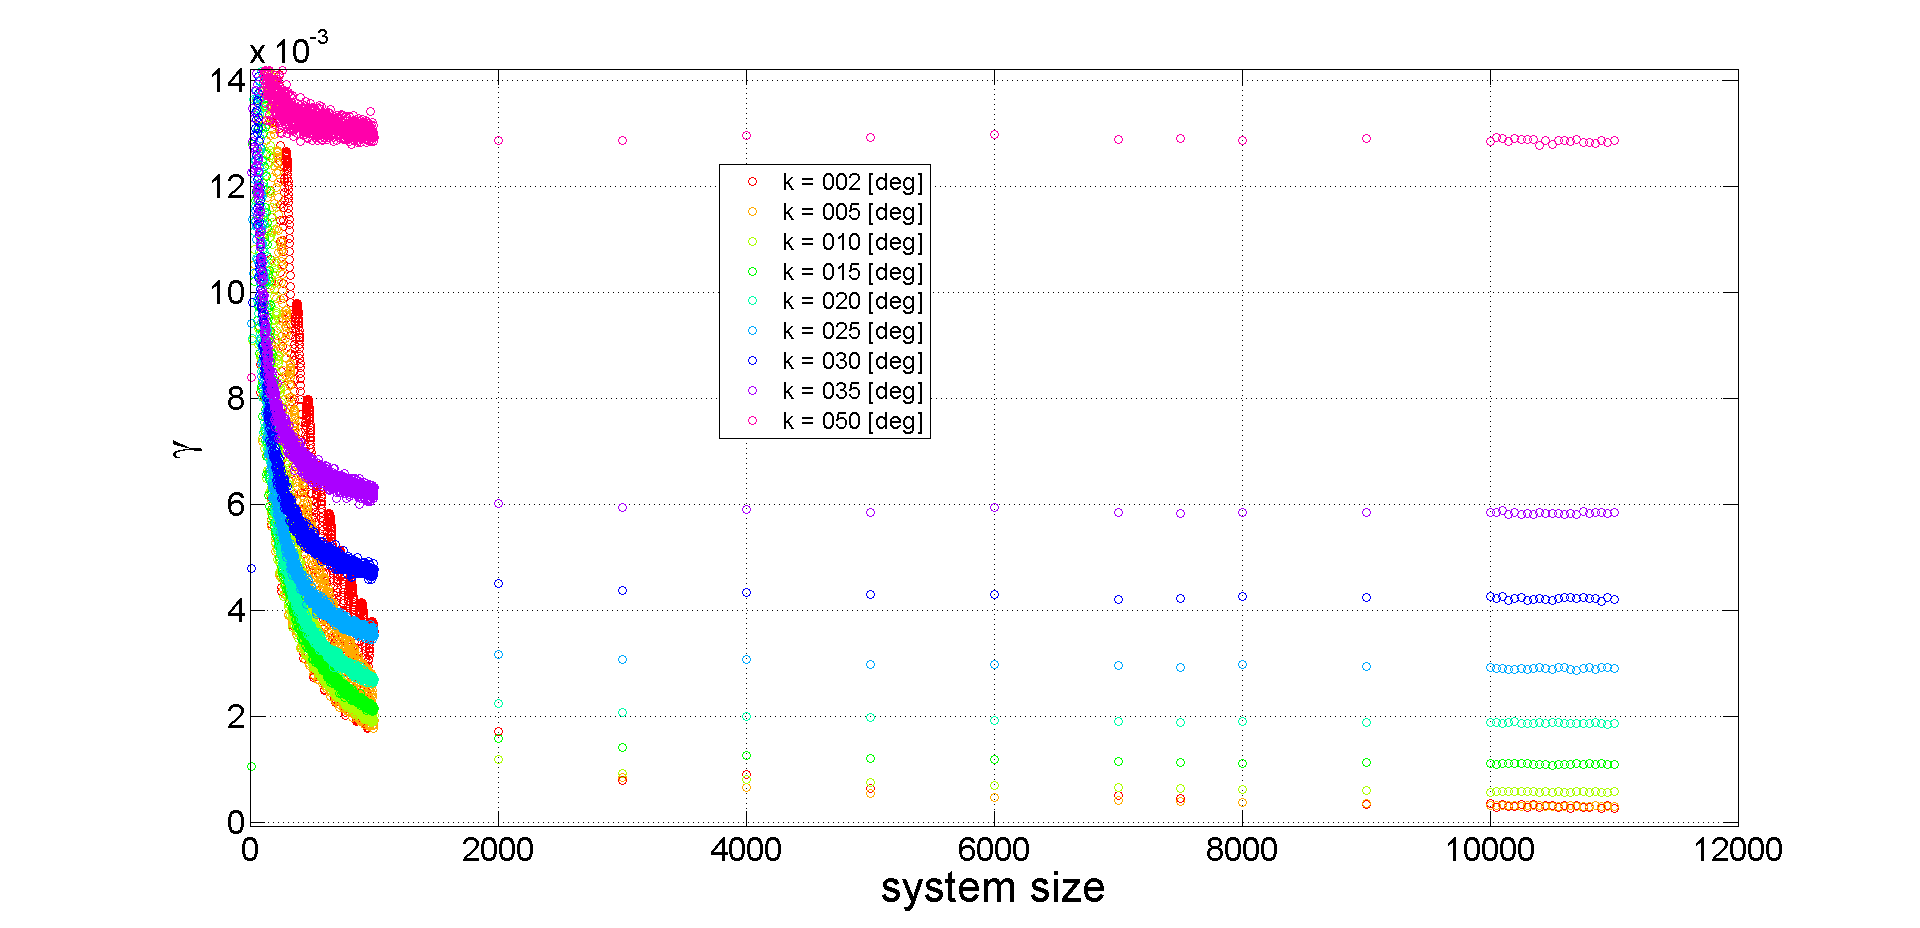
\includegraphics[width=18cm]{gamma_N2.png}
\caption{\footnotesize Asymptotic relation for different $k$s from which $\gamma$ is extracted}
\end{figure}

\subsection{Inverse localization length ($\gamma$)}
%
In the absence of disorder $\bm{W}$ describes hopping 
with some rate $w_0$, and the eigenstates are free waves labeled by~$k$. 
With disorder the~$w_0$ of the unperturbed Hamiltonian is 
loosely defined as the average~$w$. Later we shall go beyond 
the Born approximation and will show that it should 
be the harmonic average (as already defined previously).   
%
The disorder couples states that have different~$k$. 
For diagonal disorder ("pinning") the couplings are proportional to the 
variance of the diagonal elements, 
namely ${ \overline{|W_{k,k'}|^2} = (1/L)\text{Var}(v)}$.
%
For off-diagonal disorder (random spring constants) 
the  couplings are proportional to the variance  of 
the off-diagonal elements, and depends on~$b$ and on~$k$ too:
%
\beq
\overline{\left|W_{k',k}\right|^2}  =  \frac{\text{Var}(w)}{L} \ \sum_{r=1}^{b} \left[2\sin(rk'/2) \, 2\sin(rk/2)\right]^2 
\eeq
%
It follow that for small~$k$ we have ${|W_{k,k'}|^2 \propto b^5 \sigma_{\perp}^2 k^4}$. 


The Fermi-Golden-Rule (FGR) picture implies that 
the scattering rate is ${\tau^{-1}= 2\pi \varrho(\omega) \overline{\left|W_{k',k}\right|^2}}$. 
%
The Born approximation for the mean free path is ${\ell=[d\lambda/dk]\tau}$, 
where the expression in the square brackets is the group velocity 
in the electronic sense ($\lambda$ is like energy). 
The Debye approximation implies $d\lambda/dk \approx 2[c^2]k$.
% 
The inverse localization length is $\gamma=(2\ell)^{-1}$. 
From here (without taking the small $k$ approximation) it follows that 
%
\beq \label{FGRv}
\gamma(\omega) \ \ &\approx& \ \ 
\frac{1}{8}\left[\frac{9}{b^6}\right]\left(\frac{\sigma_{\parallel}}{w_0}\right)^2  \left(\frac{1}{\sin(k)}\right)^2
\\ \label{FGRw} &+& \ \ 
\frac{1}{8}\left[\frac{9}{5b}\right]\left(\frac{\sigma_{\perp}}{w_0}\right)^2  \left( 2\tan\left(\frac{k}{2}\right) \right)^2
\eeq
%
where the prefactors in the square brackets assume ${b\gg1}$, and should be replaced by unity for ${b=1}$.
In the absence of pinning the localization length diverges ($\gamma \propto k^2$) 
at the band floor, as assumed by Debye. This behavior is demonstrated in \Fig{f2} 
for two types of glassy disorder. The deviations from \Eq{FGRw} 
will be explained in the next paragraphs. 




% gamma vs $k$, box disorder
%%%%%%%%%%%%%%%%%%%%%%%%%
\begin{figure}

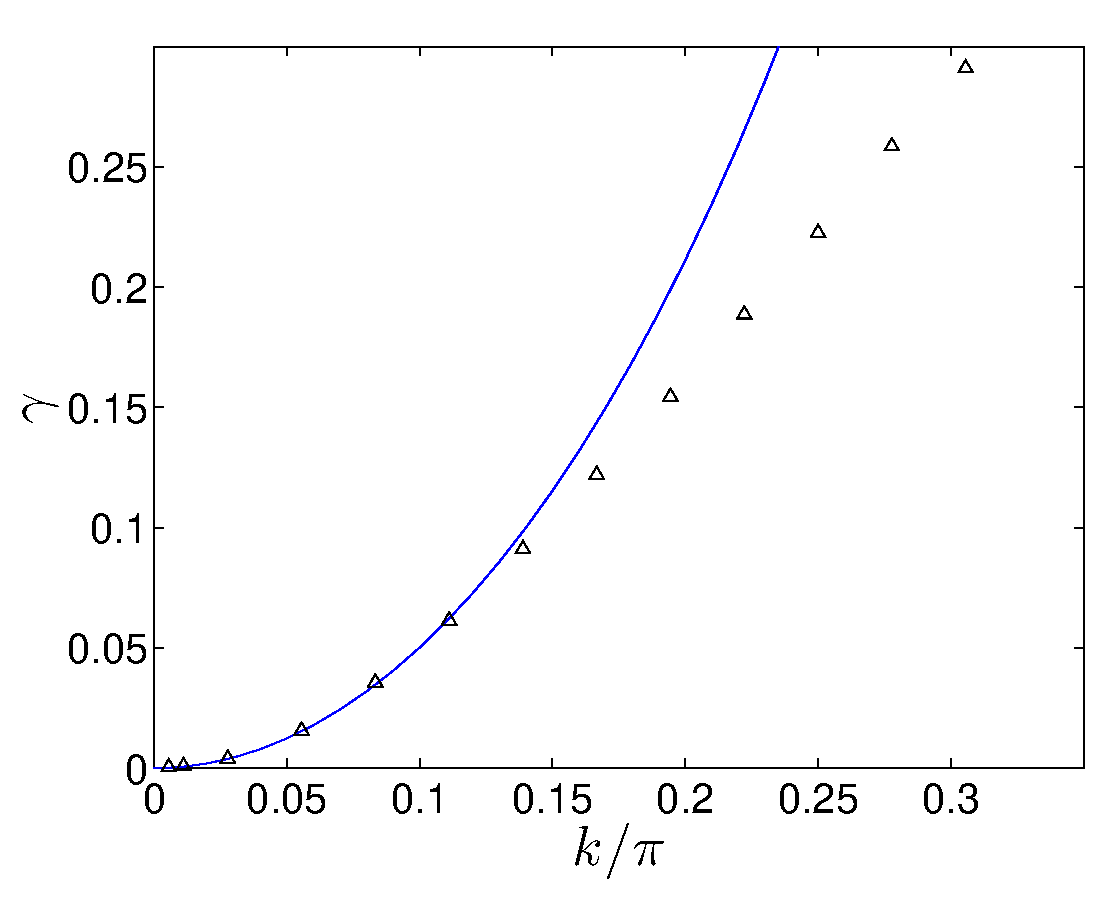
\includegraphics[width=4cm]{gammaVSkBX}
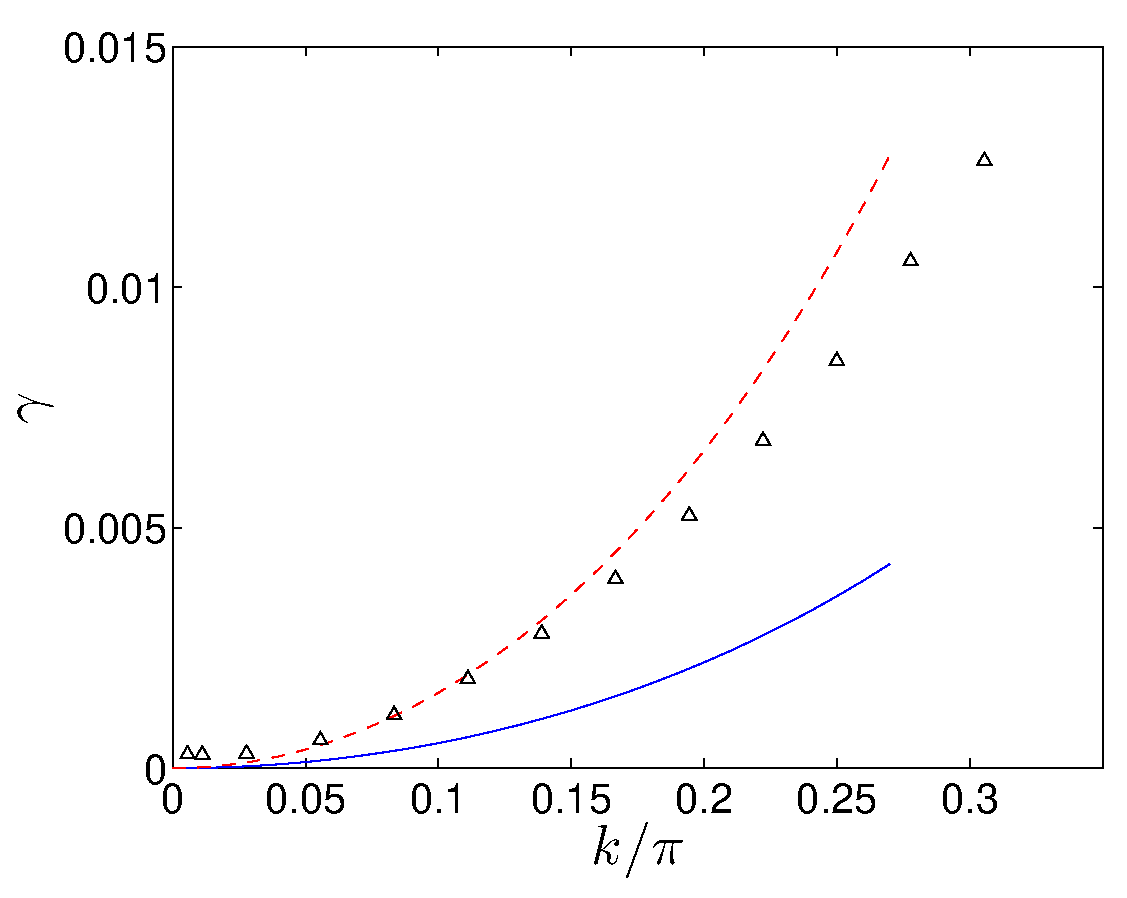
\includegraphics[width=4cm]{gammaVSkPL}

\caption{The inverse localization length $\gamma$ versus $k$ 
for logbox distributed rates with $\sigma=10$ (a);   
and for powerlaw distributed rated with $s=4$ (b).  
Pure off-diagonal disorder is assumed.
The numerical results here and in the next figure 
are based on the transfer matrix method (symbols), 
with several hundreds of realizations up to ${L\sim10^4}$.
They are compared to the naive Born expectation \Eq{FGRw} (solid blue line).
In panel (b) the upper dashed red line is based on our improved 
estimate for ``glassy disorder"  \Eq{e12}, 
while in (a) it coincides with the naive estimate (hence not indicated). 
The inverse localization length $\gamma$ is over-estimated 
as $k$ becomes larger due to the Lifshitz tail anomaly (see text).  
}
\label{f2}
\end{figure}





%%%%%%%%%%%%%%%%%%%%%%%%%%%%%%%%%%%%%%%%%%%%%%%%%%%%%%%%%%

%
The Born approximation has assumed weak disorder. 
Here we would like to consider the more general case 
of glassy disorder. For this purpose we write 
the equation ${\bm{W}\psi = \lambda \psi}$ for the eigenstates 
as a map of a single variable ${r_n=\psi_{n}/\psi_{n-1}}$,   
namely  ${r_{n+1} = -R_n/r_n - A_n}$,  
where ${R_n=w_{n-1}/w_{n}}$, and ${A_n = (\lambda-v_n-w_n-w_{n-1})/w_n}$.
In the case of diagonal disorder it takes the from  
%
\be{8}
r_{n+1} \ = \ -\frac{1}{r_n} - \epsilon + f_n
\eeq
%
where $f_n=v_n/w_0$ is the scaled disorder 
and $\epsilon=(\lambda/w_0){-}2 \equiv 2\cos(k)$ 
is the scaled energy 
measured from the center of the band.
%
Without the random term $f_n$ this map has a fixed-point 
that is determined by the equation ${ r^2+\epsilon r +1=0 }$, 
with elliptic solution for ${\epsilon\in[-2,2]}$. 
The random term is responsible for having 
a non zero inverse localization length.
The Born approximation \Eq{FGRv} is written as  
%
\be{9}
\gamma \ \ = \ \ -\langle \ln(r) \rangle \ \ \approx \ \ \frac{1}{8} \, \frac{ \mbox{Var}(f)}{\left[1-(\epsilon/2)^2\right]}
\eeq
% 
This standard estimate does not hold close to the band-edge $\epsilon_0{=}{-}2$. 
The energy scale that controls the so-called Lifshitz tail region 
is $\epsilon_c = [\mbox{Var}(f)]^{2/3}$.
In the region $|\epsilon-\epsilon_0|<\epsilon_c$ the inverse localization 
length has finite value $\gamma \sim \sqrt{\epsilon_c}$.
This observation has no dramatic consequences at this stage 
since we assume a weak pinning potential. 


%%%%%%%%%%%%%%%%%%%%%%%%%%%%%%%%%%%%%%%%%%%%%%%%%%%%%%%%%%
%
We now turn to consider the glassy disorder due to the dispersion of the $w_n$. 
Here we cannot trust the Born approximation because a small parameter is absent. 
However, without any approximation we can write the map in the form 
%
\be{10}
r_{n+1} \ \ = \ \ R_n \left( 1 - \frac{1}{r_n}\right) + 1 -\frac{\lambda}{w_n} 
\eeq
%
For $\lambda{=}0$ the zero momentum state is a solution as expected, 
irrespective of the disorder: the randomness in $R_n$ is not effective 
in destroying the ${r=1}$ fixed point. Therefore, for small $\lambda$, 
we can set without much error ${R_n=1}$. The formal argument that justifies 
this approximation is based on the linearization ${(r_{n+1}-1)=R_n(r_n-1)}$, 
and the observation that the product ${R_1R_2R_3...}$ remains of order unity. 
On the basis of this insight \Eq{e10} reduces to \Eq{e8} with the identifications 
%
\beq
\epsilon = -2 + \frac{\lambda}{w_0}, 
\ \ \ \ \ f_n = -\lambda \left(\frac{1}{w_n}-\frac{1}{w_0} \right)
\eeq 
%
The expression for~$\epsilon$ justifies the identification of the harmonic average $w_0$ 
as the effective coupling. Furthermore, we observe that there is an {\em emergent} small parameter, 
namely, the dispersion of~$f$, which is proportional to $\lambda$ irrespective of the glassiness. 
Thus we have deduced a {\em duality} between ``strong" glassy disorder and ``weak" diagonal disorder.
%
In the context of the dual problem we can use with confidence the Born approximation \Eq{e9}, leading to  
%
\be{12}
\gamma \ \ \approx \ \ \frac{1}{8} w_0^2 \, \mbox{Var}\left(\frac{1}{w}\right)  
\, \frac{4\left(\frac{\lambda}{2w_0}\right)}{2-\left(\frac{\lambda}{2w_0}\right)}
\eeq
% 
This would coincide with the primitive Born approximation \Eq{FGRw} 
if we could replace the harmonic averages by algebraic averages, namely,  
%
\beq
\frac{\mbox{Var}(1/w)}{\langle 1/w \rangle^2} 
\ \ \mapsto \ \ 
\frac{\mbox{Var}(w)}{\langle w \rangle^2} 
\eeq 
%
For log-box distribution the two types of averages provide exactly the same result, but for 
power-law disorder the two prescriptions differ enormously. This is demonstrate in \Fig{f2}, 
were we present our numerical results together with the theoretical predictions. 
%
Irrespective of that, the inverse localization length $\gamma$ is over-estimated as $k$ becomes larger. 
We can trace the origin of this discrepancy to the Lifshitz anomaly in the Anderson model.
The condition ${|\epsilon-\epsilon_0|<\epsilon_c}$ translates into ${\lambda > w_0^{-3}[\mbox{Var}(1/w)]^{-2}}$.
Thus the anomaly develops not at the band floor but as we go up in~$\omega$, 
where the inverse localization length becomes $\gamma \propto \omega^{4/3}$ 
instead of $\gamma \propto \omega^2$. 



% var[ln(g)] and ln<g> vs <ln(g)>
%%%%%%%%%%%%%%%%%%%%%%%%%%%%%%%%%%%%%%%%%%%

\begin{figure}

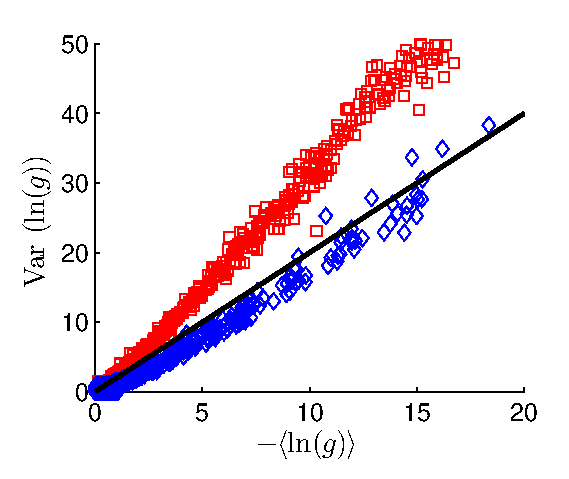
\includegraphics[clip,width=4cm]{varVSavg}
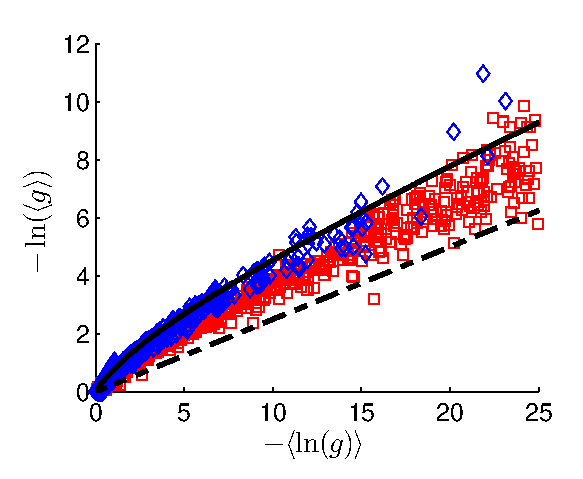
\includegraphics[clip,width=4cm]{avgVSavg}

\caption{ \footnotesize 
Testing one parameter scaling for glassy disorder. 
The variance of $\ln(g)$ (left panel) and the log of the average $-\ln\langle g \rangle$ (right panel)
are plotted against the scaling parameter $-\langle \ln(g) \rangle$. 
The calculation is done for powerlaw distributed rates 
with ${s=15}$ (blue diamonds) and ${s=1.2}$ (red squares).
The solid line is the standard one parameter scaling prediction for weak disorder, 
and the dashed line is its asymptotic approximation. 
One observes that an anomaly develops as the disorder becomes glassy.}

\label{f3}
\end{figure}


\begin{thebibliography}{99}

\bibitem{LLP03} 
S. Lepri, R. Livi, \& A. Politi, 
%{\em Thermal conduction in classical low-dimensional lattices},
Phys. Rep. {\bf 377}, 1 (2003).

\bibitem{D08} 
A. Dhar, 
%{\em Heat transport in low-dimensional systems}, 
Adv. Phys. {\bf 57}, 457 (2008).

\bibitem{LRWZHL12} 
N. Li, J. Ren, L. Wang, G. Zhang, P. H\"anggi, and B. Li, 
%{\em Colloquium: Phononics: Manipulating heat flow with electronic analogs and beyond}, 
Rev. Mod. Phys. \textbf{84}, 1045 (2012).


\bibitem{COGMZ08}
C.W. Chang, D. Okawa, H. Garcia, A. Majumdar,  A. Zettl, 
%{\em Breakdown of Fourier’s Law in Nanotube Thermal Conductors}, 
Phys. Rev. Lett, {\bf 101}, 075903 (2008).

\bibitem{NGPB09} 
D.L. Nika, S. Ghosh, E. P. Pokatilov, and A. A. Balandin, 
% {\em Lattice thermal conductivity of graphene flakes: Comparison with bulk graphite}, 
Appl. Phys. Lett. {\bf 94}, 203103 (2009).


\bibitem{ZL10} 
G. Zhang, B. Li,
% {\em Impacts of Doping On Thermal and Thermoelectric Properties of Nan-Materials"},  
NanoScale {\bf 2}, 1058 (2010).

\bibitem{K1} 
H. Li, T. Kottos, B. Shapiro, 
% Thermal transport in phononic Cayley-tree networks
Phys. Rev. E  91, 042125 (2015).

\bibitem{K2} 
M. Schmidt, T. Kottos, B. Shapiro,
% Random-matrix-theory approach to mesoscopic fluctuations of heat current
Phys. Rev. E  88, 022126 (2013).

\bibitem{D01}
A. Dhar, 
% {\em Heat Conduction in the Disordered Harmonic Chain Revisited}, 
Phys. Rev. Lett. {\bf 86}, 5882 (2001).

\bibitem{LXXZL12} 
S. Liu, X. Xu, R. Xie, G. Zhang, B. Li, 
% Anomalous Heat Conduction and Anomalous Diffusion in Low Dimensional Nanoscale Systems
Euro. Phys. J. B 85, 337 (2012).
% arXiv:1205.3065v2 [cond-mat.stat-mech] (2012).

\bibitem{DL08} 
A. Dhar, J.L. Lebowitz, 
Phys. Rev. Lett. {\bf 100}, 134301 (2008).

\bibitem{LD05} 
L. W. Lee, A. Dhar, 
Phys. Rev. Lett. {\bf 95}, 094302 (2005).

\bibitem{RD08} 
D. Roy, A. Dhar, 
Phys. Rev. E {\bf 78}, 051112 (2008).

\bibitem{LZH01} 
B. Li, H. Zhao, B. Hu, 
Phys. Rev. Lett. {\bf 86}, 63 (2001).

\bibitem{KCRDLS10a}
A. Kundu, A. Chaudhuri, D. Roy, A. Dhar, J.L. Lebowitz, H. Spohn,
Europhys. Lett. {\bf 90}, 40001 (2010).

\bibitem{KCRDLS10b}
A. Chaudhuri, A. Kundu, D. Roy, A. Dhar, J.L. Lebowitz, H. Spohn,
% Heat transport and phonon localization in mass-disordered harmonic crystals
Phys. Rev. B {\bf 81}, 064301 (2010).

\bibitem{BZFK13}
J.D. Bodyfelt, M. C. Zheng, R. Fleischmann, T. Kottos, 
Phys. Rev. E {\bf 87}, 020101(R) (2013)

\bibitem{DG84}
B. Derrida and E. Gardner, 
J. Physique {\bf 45}, 1283 (1984). 

\bibitem{Abrikosov}
A.A. Abrikosov, 
% The paradox with the static conductivity of a one-dimensional metal,
Solid State Communications {\bf 37}, 997 (1981)

\bibitem{Shapiro}
B. Shapiro, 
%Probability distributions in the scaling theory of localization
Phys. Rev. B 34, R4394 (1986)
%http://journals.aps.org/prb/abstract/10.1103/PhysRevB.34.4394


\bibitem{Izrailev}
F.M. Izrailev, A.A. Krokhin, N.M. Makarov,
%Anomalous localization in low-dimensional systems with correlated disorder
Physics Reports 512, 125 (2012).
% http://www.sciencedirect.com/science/article/pii/S0370157311002936

\bibitem{dubi}
Y. Dubi, M. Di Ventra,
%Fourier’s law: Insight from a simple derivation
Phys. Rev. E 79, 042101 (2009).
% http://journals.aps.org/pre/abstract/10.1103/PhysRevE.79.042101

\bibitem[a]{rmrkA}
Given an eigenstate $\psi$ we define $p_n=|\psi_n|^2$.
The normalization is such that $\sum p_n=1$. 
The participation number PN$=[\sum p_n^2]^{-1}$ 
is a measure for the number of sites that are occupied 
by the eigenstate.

\end{thebibliography}

\end{document}

